
\chapter{Background}
\label{chap:background}

We introduce in this chapter the most important concepts and methods employed in the field of spoken dialogue systems, with special emphasis on dialogue management.  We start by reviewing some key linguistic concepts that are particularly relevant for our work: turn-taking, dialogue acts and grounding.  A proper understanding of these aspects is indeed a prerequisite for the design of conversationally competent dialogue systems. After this linguistic overview, we move to a more technical discussion of the software architectures used to implement practical dialogue systems.  These architectures typically comprise multiple processing components, from speech recognition to understanding, dialogue management, output generation and speech synthesis.  We briefly describe the role of each component and their positions in the global processing pipeline. 

Last but not least, the final section of this background chapter delves into the diverse set of approaches that have been put forward to tackle the dialogue management problem.  We first present hand-crafted approaches, starting with finite-state policies and pursuing with more sophisticated methods based on logic- or plan-based reasoning.  Finally, we survey the more recently developed statistical approaches to dialogue management that seek to automatically extract dialogue strategies from data, based on supervised and reinforcement learning methods.

\section{What is spoken dialogue?}

We communicate in order to fulfil a wide array of social functions, such as exchanging ideas, recollecting experiences,  sustaining relationships, or collaborating with others to accomplish shared goals. These communication skills are developed in early childhood, and our cognitive abilities are in many ways shaped and amplified by this disposition for verbal interaction.  

One of the most important property of dialogue is that it is fundamentally a \textit{collaborative activity} (emphasis on both terms).  It is, first of all, an \textit{activity}, which means that is is (1) motivated by the desire to achieve specific (practical or social) goals; (2) subject to costs to minimise (the communication effort); and (3) composed of a temporal sequence of basic actions.  Furthermore, if we abstract from so-called ``internal dialogues'' with oneself, dialogue involves per definition at least two participants that must act together to keep the dialogue on track.  As shown by a wealth of studies in psychology and linguistics \citep{Clark1989,Allwood92,Clark96,Garrod2004,Tomasello2005}, human conversations are characterised by a high degree of \textit{collaboration} between interlocutors.  The individuals participating in a dialogue routinely collaborate in order to coordinate their contributions and ensure mutual understanding, thereby making the interaction more efficient. This collaboration is done mostly unconsciously and is part and parcel of the conversational skills we develop as speakers of a given language. 

We describe in the next sections four major aspects of this collaborative activity: \begin{enumerate}
\item The dialogue participants take \textit{turns} in a conversation.
\item These turns are structured into basic communicative units called \textit{dialogue acts}.
\item The interpretation of these dialogue acts is subordinated to the \textit{conversational context} in which they are uttered. 
\item The participants continuously provide \textit{grounding signals} to each other in order to indicate how they understand (or fail to understand) each other's contributions.
\end{enumerate}

\subsection{Turn-taking}

Turn-taking\index{turn-taking} is one of the most basic (yet often neglected) aspect of spoken dialogue. The physical constraints of the communication channel impose that participants take turns in order to speak.   Turn-taking is essentially a resource allocation problem.  In this case, the resource to allocate is called the \textit{conversational floor}\index{conversational floor}, and social conventions dictate how the dialogue participants are to take and release their turns. 

The field of  \textit{conversation analysis}\index{conversation analysis} studies what these conventions are and how they combine to shape conversational behaviours. Human conversations are indeed remarkably efficient at turn-taking.  Empirical cross-linguistic studies have shown that the average transition time between turns revolves around 250 ms. \citep{Stivers30062009}.\footnote{Interestingly, this duration is shorter than the time required for a human speaker to plan the motor routines associated with the physical act of speaking.  This means that the next speaker must start planning his utterance before the current turn is complete, and predict when a potential turn boundary is likely to appear.} In addition, most of the utterances do not overlap: \cite{Levinson1983} indicates that less than 5 \% of the speech stream contains some form of overlap in spontaneous conversations.  

A wide variety of cues are used to detect turn boundaries, such as silence, hesitation markers, syntax (complete grammatical unit), intonation (rising or falling pitch) and body language, as described by \cite{Duncan1972}.   These cues can occur jointly or in isolation. Upon reaching a turn boundary, a set of social conventions governs who is allowed to take the turn.  The current speaker can explicitly select the next person to take the turn, for instance when greeting someone or asking a directed question \citep{sacks1974}.   This selection can also occur via other mechanisms such as gaze.  When no such selection is indicated, other participants are allowed to take the turn.  Alternatively, the current speaker can continue to hold the floor until the next boundary. 

Turn-taking is closely related to the notion of \textit{initiative}\index{initiative} in human--computer interaction. The vast majority of dialogue systems currently deployed are either system-initiated or user-initiated.  In a system-initiated dialogue, the dialogue system has full control on how the interaction is unfolding -- i.e. the system is asking all the questions and waiting for the user responses.  A user-initiated dialogue is the exact opposite: in such settings, the user is assumed to lead the interaction and request information from the system.  The most complex -- but also most natural -- interaction style is the mixed-initiative\index{mixed initiative}, where both the user and the dialogue system are allowed to take the initiative at any time and decide to either provide or solicit information whenever they see fit \citep{Horvitz:1999}. 

The turn-taking behaviour of most current-day dialogue systems remains quite rudimentary.  The most common method to detect the end of a user turn is to wait for a silence longer than a manually fixed threshold, typically ranging between 
\textonehalf  $ $ and 1.0 second.  Some system architectures also include routines for handling barge-ins\index{barge-in} -- that is, user interruptions --  \citep{StromS00}, while others simply ignore them altogether. Turn-taking has recently become a focus of research in its own right in the dialogue system literature \citep{RauxE09,Gravano2011}, in an effort to break away from the ping-pong interaction style that characterises most current dialogue interfaces.  

\subsection{Dialogue acts}

Each turn is constituted of one or more utterances.  As argued by \cite{Austin1962} and \cite{Searle1969}, utterances are nearly always purposeful: they have specific goals and are intended to provoke a specific psychological effect on the listener(s).  They are therefore best described as actions rather than abstract statements about the world.  The notion of dialogue act\index{dialogue act} embodies precisely this idea.\footnote{Dialogue acts have gone through multiple names over time, owing to the diverse range of research fields that have studied them, from philosophy to descriptive and computational linguistics.  As listed in \cite{mctear2004}, alternative denominations include speech acts \citep{Searle1969}, communicative acts \citep{allwood1976}, conversation acts \citep{TraumH92}, conversational moves \citep{sinclair1975}, and dialogue moves \citep{LarssonCEL99}.} \cite{Bunt1996} defines a dialogue act as a ``functional unit of a dialogue used by the speaker to change the context''.

In his seminal work on the philosophy of language, \cite{Searle1979} established a taxonomy of speech acts\index{speech act} divided in five central categories:
\begin{description}
\item[Assertives: ] Committing the speaker to the truth of a proposition. \\
Examples: \utt{I swear I saw him on the crime scene.}, \utt{I bought more coffee.}
\item[Directives: ]  Attempts by the speaker to get the addressee to do something. \\ Examples:  \utt{Clean your room!}, \utt{Could you post this for me?}
\item[Commissives: ] Committing the speaker to some future course of action. \\ Examples: \utt{I will deliver this review before Monday.}, \utt{I promise to work on this.}
\item[Expressives: ] Expressing the psychological state of the speaker about a state of affairs. \\ Examples: \utt{I am so happy for you!}, \utt{Apologies for being late.}
\item[Declaratives: ] Bringing about a different state of the world by the utterance. \\ Examples: \utt{You're fired.}, \utt{We decided to let you pass this exam.}
\end{description}

Modern taxonomies of dialogue acts are significantly more detailed than the one introduced by Searle.  They also provide detailed accounts of various dialogue-level phenomena such as grounding (cf. next section) that were absent from Searle's analysis. The most well-known annotation scheme is DAMSL (Dialogue Act Markup in Several Layers\index{DAMSL}) and was initially formalised by \cite{Core1997}.  DAMSL defines a rich, multi-layered annotation scheme for dialogue acts that is both domain- and task- independent.  A modified version of this scheme was applied to annotate the Switchboard corpus\footnote{The Switchboard corpus is a corpus of spontaneous telephone conversations collected in the early 1990's.  It includes about 2430 conversations averaging 6 minutes in length; totalling over 240 hours of recorded speech with native speakers of American English \citep{Godfrey1992}.} based on a set of 42 distinct dialogue acts \citep{Jurafsky1997}, including greeting and closing actions, acknowledgements, clarification requests, self-talk, responses, and many more.  An interesting aspect of DAMSL is the use of two complementary dimensions in the markup: the \textit{forward-looking functions}\index{forward-looking function}, which are the traditional speech acts in Searle's sense (assertions, directives, information requests, etc.) and the \textit{backward-looking functions}\index{backward-looking function} that respond back to a previous dialogue act and can signal agreement, understanding, or provide answers.  Both backward- and forward-looking functions can be present in the same utterance. 

Determining the dialogue act corresponding to a given utterance is a non-trivial operation. The type of utterance only gives a partial indication of the underlying dialogue act -- a question can for instance express a directive (\utt{Could you post this for me?}).  In order to accurately classify a dialogue act, a variety of linguistic factors must be taken into account, such as prosody, lexical, syntactic and semantic features, and the preceding dialogue history \citep{jurafsky1998,Shriberg1998,stolcke2000,Keizer2007}.

\subsection{Interpretation of dialogue acts} 

Dialogue acts are strongly contextual in nature: their precise meaning can often only be comprehended within the particular conversational context in which they appear. The successful interpretation  of dialogue acts must therefore venture beyond the boundaries of the isolated utterance. We briefly review here three striking aspects of this dependence on context.

\subsubsection*{Implicatures}
\index{implicature}
As shown by \cite{Grice1989}, an important part of the semantics of dialogue acts is not explicitly stated but rather implied from the context.  Consider the following constructed example: 
\begin{center}
\begin{dialogue}
\speak{A} Is William working today?
\speak {B} He has a cold.
\end{dialogue}
\end{center}
In order to retrieve the ``suggested'' meaning behind B's utterance -- namely, that William is probably not working --, one needs to assume that B is cooperative and that his response is therefore relevant to A's question.  If an utterance initially seems to deliberately violate this principle, the listener must search for additional hypotheses required to make sense of the dialogue act. \cite{Grice1989} formalised these ideas in terms of a cooperative principle composed of four conversational maxims that are assumed to hold in a natural conversation: the maxim of quality (``be truthful''), the maxim of quantity (``be exactly as informative as required''), the maxim of relation (``be relevant'') , and the maxim of manner (``be relevant'').  These notions have been further developed by various theorists such as \cite{wilson2002relevance} and \cite{horn2008handbook}.  A computational account of these implicatures (and application to dialogue systems) is provided by \cite{benotti2010implicature}. 


\subsubsection*{Non-sentential utterances}
\label{non-sentential utterance}
\index{non-sentential utterance}
Non-sentential (also called elliptical) utterances are linguistic constructions that lack an overt predicate.  They include expressions such as  \utt{where?}, \utt{at 8 o'clock}, \utt{a bit less, thanks} and \utt{brilliant!}. Their interpretation generally requires access to the recent dialogue history to recover their intended meaning. This can lead to ambiguities in the resolution, as illustrated in these examples modified from \cite{Fernandez:2007}: \begin{itemize}
\item A: ``When do they open the new station?''  $\rightarrow$ B: ``Tomorrow'' (\textit{short answer})
\item A: ``They open the station today''  $\rightarrow$ B: ``Tomorrow'' (\textit{correction})
\item A: ``They open the station tomorrow''  $\rightarrow$ B: ``Tomorrow'' (\textit{acknowledgement})
\end{itemize}

Various accounts of non-sentential utterances have been proposed, based on e.g. discourse coherence \citep{Schlangen03theinterpretation} or interaction-oriented semantics \citep{fernandez2006non,Ginzburg2012}. Machine learning approaches have also been developed \citep{Schlangen:2005,Fernandez:2007}. 

\subsubsection*{Referring expressions}

Finally, dialogue acts are replete with linguistic expressions that refer to some aspect of the conversational context.  These references can be either deictic or anaphoric. 

A deictic marker\index{deictic marker} is a reference to an entity that is determined by the context of enunciation.  Examples of such markers are \utt{here} (spatial reference), \utt{yesterday} (temporal reference), \utt{this mug} (demonstrative), \utt{you} (reference to a person), or even pointing gestures. By their very definitions, deictic markers refer to different realities depending on the situation in which they are used: a \utt{here} uttered in a classroom differs from a \utt{here} uttered in the countryside.  

In addition, dialogue can also include anaphoric expressions -- that is, expressions that refer to an element that has been previously mentioned through the history of the dialogue. An simple example of such anaphoric expression can be seen in the question-answer pair \utt{Is William working today?} $\rightarrow$ \utt{He has a cold}, where the pronoun \utt{he} must be resolved to \utt{William}. 

The appropriate processing of deictic and anaphoric expressions is an important question in dialogue systems, and pertains both to the interpretation and production process. Multiple approaches have been pursued, relying on symbolic \citep{Eckert2000} or statistical techniques \citep{StrubeM03,Stent2010}.  Researchers have also investigated the integration of salience measures \citep{Kelleher:2004}, multimodal cues \citep{Frampton:2009,Chen:2011}, the processing of spatial referring expressions \citep{zender/etal:2009-ijcai} and the incrementality of the resolution process \citep{schlangen2009incremental,poesio2011incremental}. 

\subsection{Grounding}

Dialogue acts are executed as part of a larger collaborative activity that requires the active coordination of all conversational partners, i.e. speaker(s) as well as hearer(s).  This coordination takes place at various levels.  The first and most visible level is the content of the conversational activity.   The partners must ensure mutual understanding of each other's contribution, to control that they remain ``on the same page''.  In addition, they  also coordinate the process by which the conversational activity moves forward -- by signalling that they are attending to the person who currently holds the conversational floor and acknowledging her/his contributions to the dialogue.

As an illustration, consider this short excerpt from a conversation transcribed in the British National Corpus \citep{bnc} :

\begin{dialogue} 
\speak{Kathleen } How come they can take time off yet you can't?
\speak{Steve } $\ \ \ \ \ \ $ He's been there longer than me.
\speak{Kathleen } Oh.
\speak{Steve }  $\ \ \ \ \ \ $ I can, I might have two holidays now, two days' holiday. ...
\speak{Kathleen } Well ... I don't get that, me.
\speak{Steve }  $\ \ \ \ \ \ $ What?
\speak{Kathleen } All these two days' holiday and this, you've had Christmas.
\speak{Steve }  $\ \ \ \ \ \ $ You get two point summat\footnote{``Summat'' is slang for ``something'' in the Yorkshire region. } days per month worked
\speak{Kathleen } Oh so you should've got them for January? ...
\speak{Steve }  $\ \ \ \ \ \ $ right?
\speak{Kathleen } Yeah.
\speak{Steve }  $\ \ \ \ \ \ $ And I worked three month before Christmas so I got six point summat days
\speak{Kathleen } For Christmas.
\speak{Steve }  $\ \ \ \ \ \ $ so then I had all Christmas off.
\speak{Kathleen } Oh! \\
 $\phantom{a} \ \ \ \ \ \ \ $ Yeah I get it now. \\
 $\phantom{a} \ \ \ \ \ \ \ $ ... I thought you got Christmas off like we got Christmas off.
\speak{Steve }  $\ \ \ \ \ \ $ No. \\ 
 $\phantom{a} \ \ \ \ \ \ \ $ You gotta earn them. ... \vspace{-2mm}
 \begin{flushright}\begin{scriptsize}(\urlsmall{http://www.phon.ox.ac.uk/SpokenBNCdata/KCX.html})\end{scriptsize}\end{flushright} 
\end{dialogue} 

We can observe in this short dialogue that the interlocutors constantly rely on the \textit{common ground} of the interaction to move the dialogue forward.  They regularly check what pieces of information are mutually known and understood (e.g. \utt{right?}).  They also make use of a variety of signals to indicate when things are properly grounded (\utt{oh}, \utt{yeah}, \utt{I get it}) and when they are not (\utt{I don't get that}, \utt{what?}). The common ground\index{common ground} progressively expands as the dialogue unfolds -- for instance, the system of holiday entitlement is not initially part of the shared knowledge for both speakers at the onset of the conversation, but becomes so towards the end. 

The common ground is defined as the collection of shared knowledge, beliefs and assumptions that is established during an interaction.\footnote{An information that is part of the common ground for a given group is more than simply known by every member of the group.  All group members must also be aware that the information is shared and known by the other members. Formally speaking, a proposition $p$ is part of the common knowledge for a group of agents $G$ when all the agents in $G$ know $p$, and they also all know that they all know $p$, and they all know that they all know that they all know $p$, \textit{ad infinitum}. This definition can be formalised using the mathematical apparatus of set theory or epistemic logic \citep{meyer2004epistemic}. } Each dialogue act is built upon the current common ground and participates in its gradual expansion and refinement.  This process is called \textit{grounding}\index{grounding}.  A variety of feedback mechanisms  can be used to this effect.  As described by \cite{Clark1989}, positive evidence\index{positive feedback} of understanding can be expressed via cues such as:
\begin{description}
\item[Continued attention: ] The hearer shows that he/she continues to attend to the speaker.
\item[Relevant next contribution: ] The hearer produces a relevant follow-up, as in the answer \utt{He's been there longer than me} following the question that precedes it.
\item [Acknowledgement: ] The hearer nods or utters a backchannel such as \utt{mm}, \utt{uh-uh}, \utt{yeah}, or an assessment such as \utt{I see}, \utt{great}, \utt{I get it now}.
\item [Demonstration: ] The hearer demonstrates evidence of understanding by reformulating or completing the speaker utterance.
\item [Display: ] The hearer reuses part of the previous utterance.
\end{description}

Communication problems can also occur, owing to e.g. misheard or misunderstood utterances. The hearer should in this case provide negative feedback to signal trouble in understanding. A large panel of clarification and repair strategies\index{clarification strategy} \index{repair strategy} are available to recover from these communicative failures.  These strategies include backchannels\index{backchannel} (\utt{mm?}), confirmations  (\utt{Do you mean that...?}), requests for disambiguations, invitations to repeat, and tentative corrections.  

All in all, these positive and negative signals enable the dialogue participants to dynamically synchronise what the speaker intends to express and what the hearers actually understand.   This grounding process operates mostly automatically, without deliberate effort.  It is closely related to the concept of interactive alignment\index{alignment} that has recently been articulated by \cite{Garrod2004,Garrod2009}. Humans show a clear tendency to (unconsciously) imitate their conversational partners. In particular, they automatically align their choice of words, a phenomenon called lexical entrainment\index{lexical entrainment} \citep{brennan1996conceptual}.  But alignment also occurs on several other levels such as grammatical constructions \citep{branigan2000syntactic}, pronunciation \citep{pardo2006phonetic}, accents and speech rate \citep{giles19911}, and even gestures and facial expressions \citep{bavelas1986show}.  

A proper treatment of grounding is critical for the development of conversational interfaces.  As already mentioned in the introductory chapter, comprehension errors are indeed ubiquitous in spoken dialogue systems.  The potential sources of misunderstandings are abundant, from error-prone speech recognition to out-of-domain utterances, unresolved ambiguities, and unexpected user behaviour.  Appropriate grounding strategies are crucial to address these pitfalls. Grounding for dialogue systems is an active area of research and important advances have been made regarding the formalisation of rich computational models of grounding \citep{Traum:1994thesis,MathesonPT00}, the generation of clarification requests \citep{Purver04Thesis,Rieser:2005}, the design of human-inspired error handling\index{error handling} strategies \citep{Skantze2007}, the integration of non-verbal cues such as gaze, head nods and attentional focus \citep{Nakano:2003} and the development of incremental grounding mechanisms \citep{visser_toward_2012}.

\section{Spoken dialogue systems}
\label{sec:sds}
After reviewing some of the core properties of human dialogues, we now discuss how to develop practical computer systems that aim to emulate such type of conversational behaviour.   In the introduction chapter, Figure \ref{fig:basicsds} represented a dialogue system as a black box taking speech inputs from the user and generating spoken responses.  Real-world dialogue systems have however a complex internal structure, as we detail in the next pages.

 \subsection{Architectures}
\label{sec:architectures}

Spoken dialogue systems (SDS) often take the form of complex software architectures\index{dialogue system architectures} that encompass a wide range of interconnected components. These components are dedicated to various tasks related to speech processing, understanding, reasoning and decision-making. These tasks can be grouped into five major components: 
\begin{enumerate}
\item \textit{Speech recognition}, in charge of mapping the raw speech signal to a set of recognition hypotheses for the user utterance(s).
\item \textit{Natural language understanding}, in charge of mapping the recognition hypotheses to high-level semantic representations of the dialogue act performed by the user.
\item \textit{Dialogue management}, in charge of interpreting the purpose of the dialogue act in the larger conversational context and deciding what communicative action to perform (if any).
\item \textit{Natural language generation}, in charge of finding the best linguistic (and extra-linguistic) realization for the selected communicative action.
\item And finally, \textit{text-to-speech synthesis}, in charge of synthesizing an audio signal out of the generated utterance.
 \end{enumerate}
 \index{speech recognition}\index{dialogue understanding}\index{dialogue management}\index{natural language generation}\index{text-to-speech synthesis}
 
 Figure \ref{fig:architecture} shows the flow of information for a prototypical spoken dialogue system. Many systems rely on additional middleware to act as a ``software glue'' between the components and handle the information exchange and scheduling of modules \citep{jaspis2004,Herzog:2004,Bohus:2009,schlangen2010}.
   
 \begin{figure}[h]
\centering
\vspace{5mm}
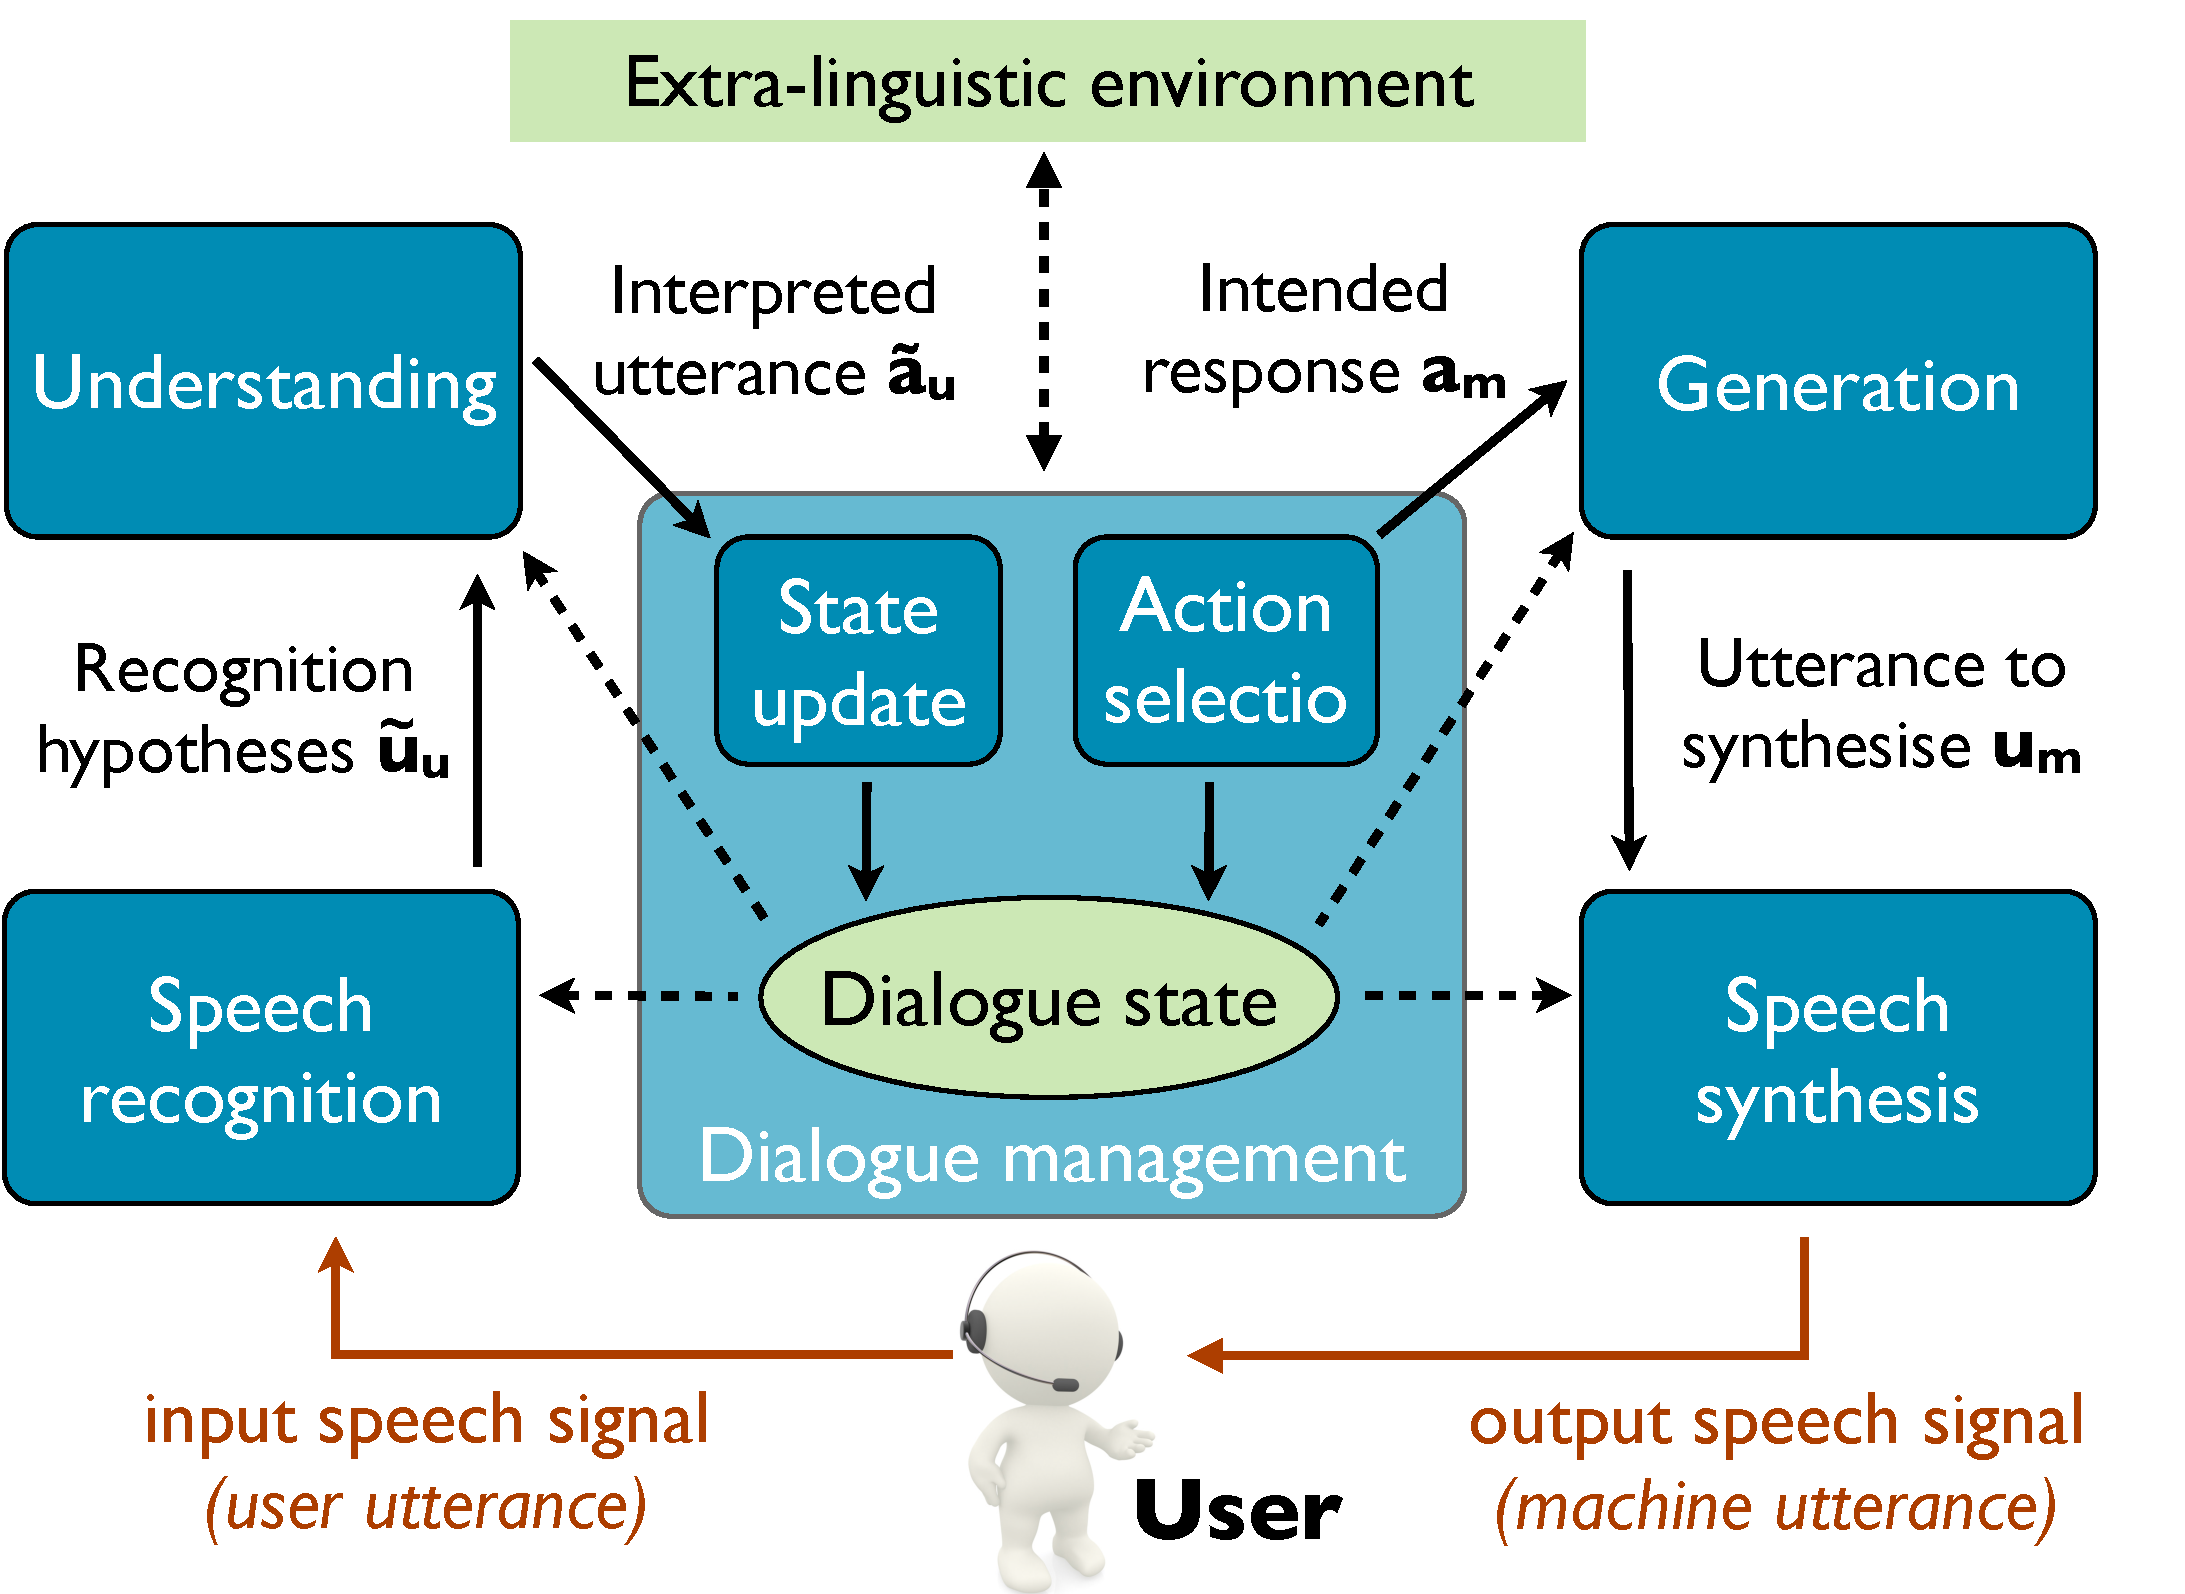
\includegraphics[scale=0.30]{imgs/architecture.pdf}
\vspace{5mm}
\caption{Information flow for a typical spoken dialogue system. The solid lines denote necessary input and outputs while the dotted lines represent optional contextual information.}
\label{fig:architecture}
\end{figure}

Spoken dialogue systems can use other modalities than speech.  In particular, additional communication channels such as touch, gestures, gaze, and other body movements can be fruitfully exploited.  As shown by e.g. \cite{smartkom}, multiple modalities can be employed to enrich communication in both directions (understanding and generation). \index{multi-modality}\index{multi-modal dialogue system}In particular, the system can refine its understanding of the actual user intentions by fusing information perceived through multiple information channels such as gestures \citep{stiefelhagen2004} or gaze \citep{koller2012}.  Non-verbal modalities can also be put to use to enhance how information is presented back to the user and convey additional grounding signals, through e.g. facial expressions and gestures. The use of multiple modalities can notably reduce understanding errors and cognitive load \citep{oviatt2004we} as well as improve the overall user experience \citep{JokinenH06}.  For all their advantages, multimodal architectures pose however a number of additional challenges related to timing, synchronisation \citep{DBLP:conf/hri/SalemKJ13} and increased system complexity. 

In addition to these non-verbal modalities, many dialogue domains are also grounded in an external context that must be accounted for\index{contextual awareness}\index{contextual modelling}.  This external context might be a physical environment for human-robot interaction, a virtual world for embodied virtual agents, a spatial location for in-car navigation systems, or simply a database of factual knowledge for information systems. Contextual factors of relevance for the application must be continuously monitored by the dialogue system (and updated whenever necessary), as many components depend on the availability of such context model for their internal processing.  Furthermore, the agent can often actively influence this context through external actions -- for instance, a grasping action will modify the location of the gripped object.   This contextual awareness necessitates the integration of additional functionalities for perception and actuation. In human--robot interaction\index{human--robot interaction} domains, these extra-linguistic modules can notably include subsystems for object and scene recognition, spatial navigation, and various motor routines for locomotion and manipulation  \citep{1570637,goodrich2007human,HawesSWZJKBBS07}. 

Several types of architectures have been proposed to assemble these components in a unified framework.  The simplest approach is to arrange the components sequentially in a pipeline\index{pipeline architecture} starting from speech recognition and ending with speech synthesis.  This approach, although relatively straightforward to develop, suffers from a number of shortcomings, amongst which the rigidity of the information flow and the difficulty of inserting feedback loops between components. Pipelines also offer poor turn-taking capabilities, since the system is unable to react before the pipeline has been fully traversed \citep{RauxE09}. More advanced architectures -- including the one put forward in this thesis -- are based on the notion of \textit{information state}\index{information state} \citep{larsson2000information,Bos2003}.  These approaches are essentially blackboard architectures revolving around a central dialogue state that is read and written by various modules connected to it.  These modules monitor the state for relevant changes, in which case they trigger their processing routines and update the state with the result.  The main advantages of such architectures are (1) a more flexible information flow, since the modules are allowed to process and update information in any order, and (2) the possibility to define modules that take full advantage of the contextual information encoded in the dialogue state.  Figure \ref{fig:architecture_comp} provides a graphical illustration of the difference between pipeline and information-state-based architectures.  

 \begin{figure}[h!]
\centering
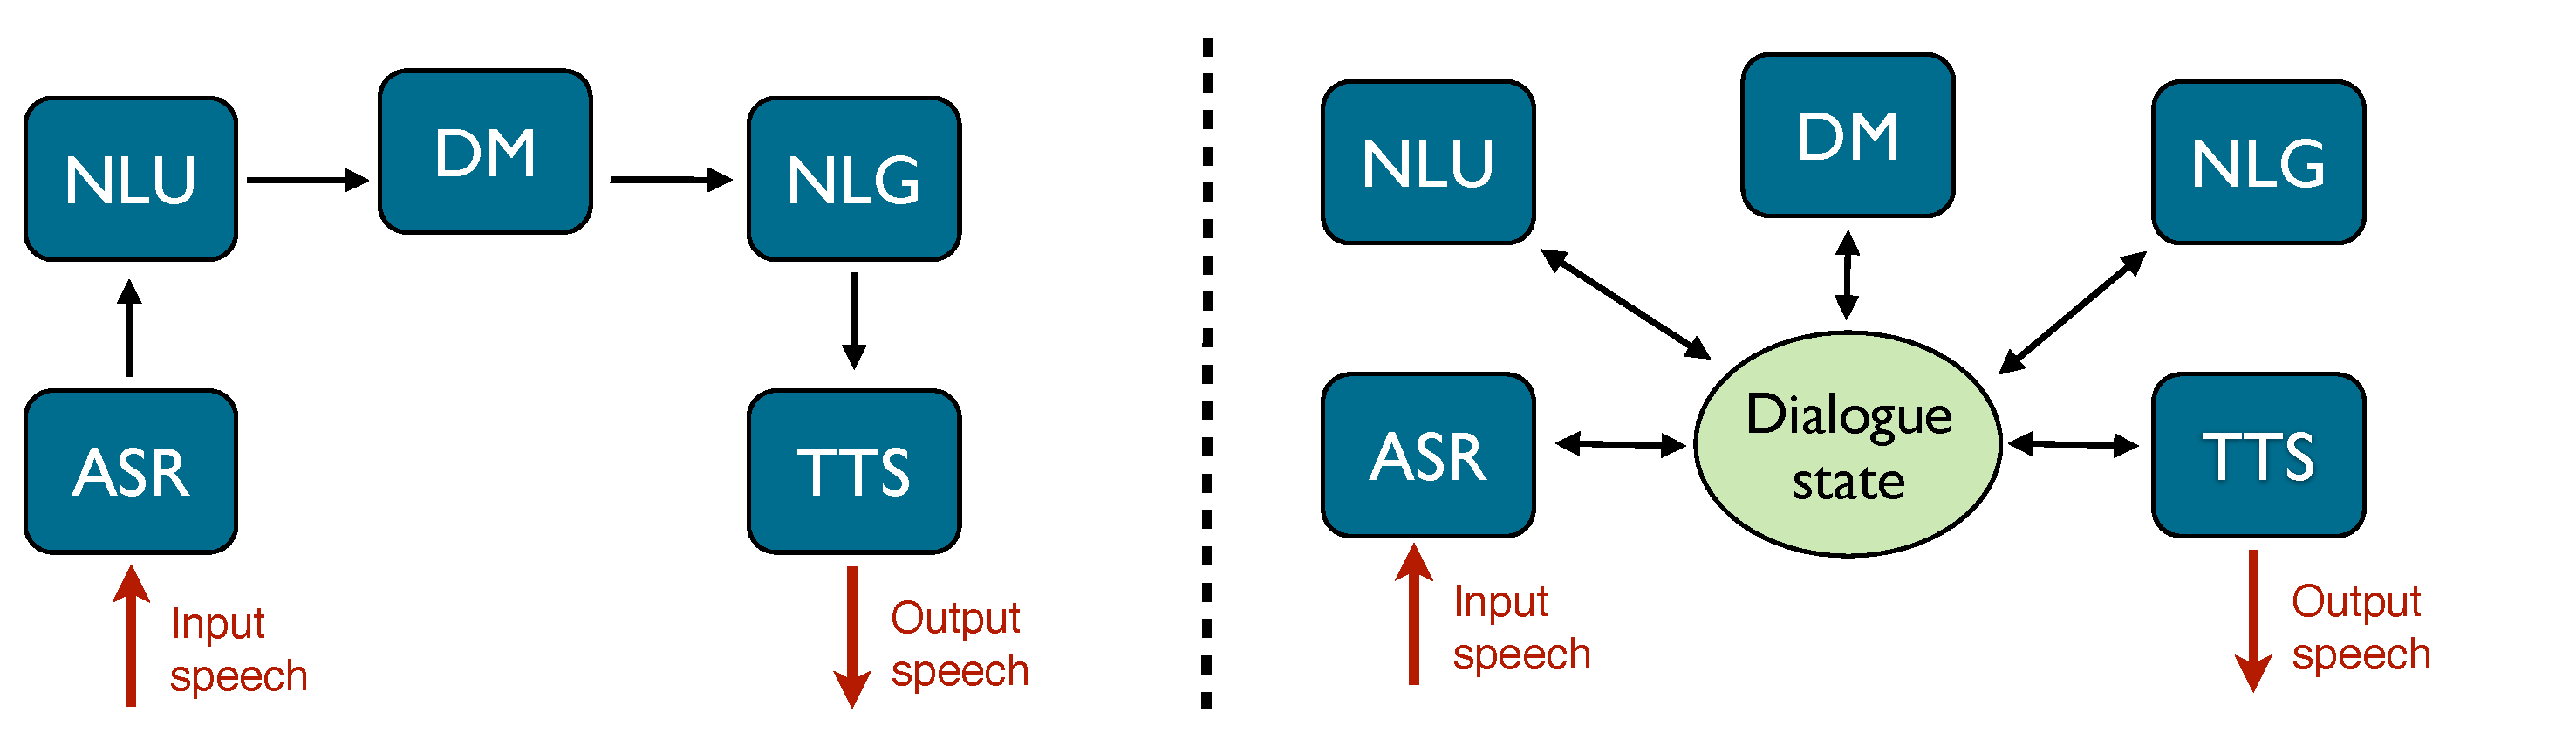
\includegraphics[scale=0.28]{imgs/architecture_comparison.pdf}
\caption{Comparison between pipeline (left) and information state (right) system architectures.   ASR = \textit{Automatic Speech Recognition}, NLU = \textit{Natural Language Understanding}, DM = \textit{Dialogue Management}, NLG = \textit{Natural Language Generation}, and TTS =\textit{Text-to-Speech Synthesis}.}
\label{fig:architecture_comp}
\end{figure}

Finally, a last aspect of dialogue system architectures that has been subject to recent research pertains to \textit{incremental processing}.  Many dialogue architectures must wait for an utterance to be fully pronounced to start its interpretation and decide on subsequent actions.  This workflow usually leads to poor reactivity and unnatural conversational behaviours.  To address this shortcoming, new architectures have been proposed to integrate incremental processing at various stages of interpretation and decision-making \citep{schlangen2009general}.\index{incremental processing}


\subsection{Components}

As explained in the previous section, the components of a dialogue systems can typically be grouped in five major steps.  We briefly describe here the role of these components and define their respective inputs and outputs.

\subsubsection*{Speech recognition}
\index{speech recognition}
Upon detection of a new speech signal emanating from the user, the first task is to recognise the corresponding utterance. Speech recognition is responsible for converting the raw speech signal from the microphone(s) into a set of hypotheses $\tilde{u}_u$ representing the words uttered by the user. To this end, the speech signal is first converted into a digital format and split into short frames (usually 10 ms). A set of acoustic features is then extracted for each frame using signal processing techniques.  Once these acoustic features are extracted, two statistical models are combined to estimate the most likely recognition hypotheses: the \textit{acoustic model} and the \textit{language model}.  \index{acoustic model}\index{language model}

The acoustic model defines the observation likelihood of particular acoustic features for a given phone\footnote{A phone is an individual sound unit of speech.  Technically speaking, acoustic models are not defined over entire phones but over sub-segments, typically decomposed into three parts: beginning, middle and end.}, while the language model defines the probability of a given sequence of words. This distinction rests on the formalisation of the speech recognition task as a \textit{Hidden Markov Model} (HMM)\index{Hidden Markov Model}, where the states represent the sequence of phones, and the observations are the acoustic features.  

%Given a sequence of acoustic observations $O$, the probability of a word sequence $W$ is straightforwardly derived using Bayes' rule: 
%\begin{equation}
%P(W|O) = \frac{P(O|W) P(W)}{P(O)} 
%\end{equation}
%where $P(O|W)$ is encoded by the acoustic model and $P(W)$ by the language model. $P(O)$ is a normalisation factor that can be ignored for decoding purposes. 

For the practical development of spoken dialogue systems, the most important element of a speech recogniser is the language model.  The language model effectively represents the set of utterances that can be accepted as inputs to the system (and their relative probabilities).  The model can be encoded either in the form of a hand-crafted recognition grammar, or via statistical modelling based on a particular corpus of reference.  In the latter case, the language model typically takes the form of an N-gram model, often a bi- or tri-gram corrected with appropriate smoothing and back-off techniques  \citep{Jelinek:1998,ChenG99}.  It is also often beneficial to dynamically modify the language model at runtime to reflect the changing context and dialogue state.  This real-time model adaptation can notably be realised by priming the words or expressions that are most contextually relevant \citep{gruenstein2005context,ESSLLI2008-springerreprint}.

The output of the speech recogniser is typically a N-best list\index{N-best list} (or recognition lattice) representing a set of possible hypotheses for the utterance, together with their relative confidence score or probabilities.  Thus, the output of the speech recogniser is a list expressed as: 
\begin{equation*}
\tilde{u}_u = \langle (\tilde{u}_u^{(1)}, p^{(1)}), (\tilde{u}_u^{(2)}, p^{(2)}), ... (\tilde{u}_u^{(n)}, p^{(n)})\rangle
\end{equation*}
where $\tilde{u}_u^{(i)}$ represents a specific recognition hypothesis and $p^{(i)}$ its corresponding probability.\footnote{In order to be proper probabilities,  the usual axioms $0 \leq p^{(i)} \leq 1$ for all $p^{(i)}$ and $\sum_{i=1}^n p^{(i)} = 1$ must be satisfied.   It should also be noted that in practice, many speech recognisers only provide raw confidence scores for their hypotheses.  Estimating the exact correspondence between these scores and meaningful probabilities is a non-trivial task that has been investigated by e.g. \cite{Williams08}.} 

\subsubsection*{Natural language understanding}
\label{section:speechunderstanding}

Once the recognition hypotheses for the utterance have been generated by the speech recogniser, the next task is to extract its semantic content.  The goal of natural language understanding (NLU) is to build a representation of the meaning(s) expressed by the form of a given utterance.  This task is a notoriously difficult endeavour, due to the combination of various factors. The first difficulty lies in speech recognition errors, with WER (Word Error Rates) often revolving around 20 \% for many dialogue applications.  The syntactic and semantic analysis of utterances is likewise complicated by the occurrence of sentential fragments,  disfluencies of various sorts (e.g. filled pauses, repetitions, corrections) and ambiguities\index{ambiguities} that must be resolved at multiple linguistic levels. 

Natural language understanding can be decomposed in a number of steps.  Parsing corresponds to the task of extracting the syntactic structure of the utterance and mapping it to a semantic representation.  Spoken language parsing can be realised through various techniques, from keyword or concept spotting \citep{KomataniTKK01,ZhangZY07} to shallow semantic parsing \citep{Coppola:2009}, grammar-based parsing \citep{VanNoord1999} and statistical parsing \citep{He200585}.  It has been shown useful to apply upstream preprocessing techniques to correct speech recognition errors \citep{Ringger:1996} and filter out disfluencies \citep{Johnson:2004}. In addition, referring expressions might also need to be resolved \citep{Funakoshi:2012}.  Finally, the dialogue act associated with the utterance must be determined \citep{stolcke2000,Keizer2007}. \cite{demori2008} provides a survey of the various models and techniques used in the field of spoken language understanding. 

Given speech recognition hypotheses $\tilde{u}_u$ given as inputs, and possibly a representation of the dialogue history and external context, the task of natural language understanding is to extract a corresponding N-best list of dialogue act hypotheses $\tilde{a}_u$ defined as: \begin{equation*}
\tilde{a}_u = \langle (\tilde{a}_u^{(1)}, p^{(1)}), (\tilde{a}_u^{(2)}, p^{(2)}), ... (\tilde{a}_u^{(n)}, p^{(n)})\rangle
\end{equation*}
where $\tilde{a}_u^{(i)}$ represents a dialogue act hypothesis, usually represented in a logical form with various predicates and arguments, and $p^{(i)}$ its corresponding probability.

\subsubsection*{Dialogue management}
\index{dialogue management}

Dialogue management occupies a central stage in spoken dialogue systems.  As already mentioned in the introductory chapter, dialogue management serves a double role.  The first task of the dialogue manager is to maintain a representation of the current dialogue state\index{dialogue state} and update it as new information becomes available\index{dialogue state update}.\footnote{Some approaches explicitly distinguish between two types of management tasks: task management, responsible for monitoring and advancing the execution of the application objectives, and dialogue management \textit{stricto sensu}, responsible for the more conversational aspects of the interaction. Establishing the boundary between the two types of tasks is however not always trivial.} This dialogue state should encode every information that is of general relevance for the system, such as the recent dialogue history (encoded as a temporally ordered sequence of dialogue acts performed by the dialogue participants), the current conversational floor, the status of the task(s) to fulfil, and various features describing the context of the interaction.  Furthermore, the dialogue state can also include information that is indirectly inferred from the individual observations. In particular, many dialogue domains include a variable that explicitly encode the hypothesised user intention.  This user intention, although never directly observed, can often be derived from the user inputs through a sequence of reasoning steps.  Similarly, the dialogue state can also integrate features that characterise the user profile and her/his preferences.\index{user model} Depending on the theoretical premises chosen for the system, the dialogue state can be either encoded as a fully observable data structure or represent partial observability through the definition of probability distributions on the values of the state variables. 

The second task of dialogue management is to take decisions based on this dialogue state.  This task is often called \textit{action selection}. \index{action selection} The dialogue manager is responsible for selecting the next action to perform by the system, which can be a communicative action (e.g. a piece of information to communicate, a question to task, a grounding signal to convey), an external action (e.g. a physical movement for a robot or a database manipulation for a booking system), a combination of the two, or no action at all.  The action selection mechanism can take many forms, ranging from a direct mapping between states and actions to the application of logical rules or the use of offline or online planning techniques. 

Dialogue management leads to two distinct outcomes: (1) an updated dialogue state that reflects the observations received as inputs (user dialogue acts, contextual changes etc.), and (2) a selected system action denoted as $a_m$ (the $m$ subscript standing for ``machine'' to distinguish it from the user act $a_u$).  As for the user dialogue act $a_u$, the system action $a_m$ is often represented in a logical form composed of predicates and arguments. 

Section \ref{sec:dm} describes in more detail the various approaches and techniques that have been proposed in the literature to formalise the dialogue management process. 

\subsubsection*{Generation}
\index{natural language generation}
Assuming the selected system action $a_m$ relates to a verbal action, the following step is to find the best linguistic realisation for the abstract communicative goal defined in $a_m$.  As for natural language understanding, a variety of generation techniques are available, from shallow generation strategies based on canned sentences or templates to more more sophisticated approaches based on sentence planning and surface realisation \citep{Stone2003,koller-stone:2007}.  More recently, statistical methods have also been pursued in enhance the robustness and user-adaptivity of the generation algorithms \citep{Rieser:2010,DethlefsC11}. 

The inputs of the generation module are the selected system action $a_m$ and optionally the features defined in the dialogue state $s$ (e.g. the user model and the external context). Given this information, the generation module will produce a corresponding user utterance denoted $u_m$.  In the case of multimodal systems, the module may also deliver realisations for other modalities than the speech channel, such as gestures or facial expressions.

\subsubsection*{Speech synthesis}
\index{text-to-speech synthesis}\index{speech synthesis}
The final step of the processing cycle is to synthesise the utterance in a speech waveform --  a process called \textit{text-to-speech synthesis}.  This synthesis is performed in two consecutive stages.  The utterance is first converted into a phonemic representation. This conversion involves multiple processing steps related to text normalisation, phonetic and prosodic analysis.  Once the conversion is completed, the resulting phonemic representation is fed to a synthesiser in charge of producing the actual waveform. This synthesis can either be performed by gluing together pre-recorded units of speech from a speech database (concatenative synthesis) or by generating sounds using explicit acoustic models of the vocal tract (formant and articulatory synthesis). Most current dialogue systems rely on concatenative synthesis, and in particular unit selection \citep{hunt1996}. 

\subsection{Applications}

Spoken dialogue systems have a wide variety of applications, ranging from academic research prototypes to mature commercial products. The first applications can be found in telephone-based systems for information access and service delivery.  A large variety of systems have been developed in this area, for applications as diverse as automated call-routing \citep{GorinRW97}, travel planning \citep{walker2001}, weather updates \citep{jupiter}, bus schedule retrieval \citep{RauxLBBE05} or tourist information \citep{lemon2006}.  The recent emergence of smartphones also led to the development of new voice interfaces for multimodal local search \citep{EhlenJ13}, cross-lingual communication \citep{yochina} and even pedestrian exploration  \citep{janarthanam2012integrating}.  Many of these ideas have found their way into commercial products, as evidenced by the success of applications such as Apple's Siri, Nuance's Dragon Go! and Google Now. 

Spoken dialogue systems can also be applied in domains where the use of touch interfaces and screens should be avoided because it is impractical or dangerous.  This is notably the case for in-car navigation systems \citep{cumove,CastronovoMPM10} where voice interfaces are to be preferred for safety reasons.  The recent trends towards ubiquitous computing and ``ambient'' intelligence in smart home environments also offer promising applications of dialogue system technology \citep{vipperla2009a,ambient2010}.

Spoken dialogue systems are deployed in increasingly complex and open-ended interaction domains, where the artificial agent is no longer a mere executor of user commands, but increasingly plays the role of a collaborator or intelligent assistant.  Conversational interfaces have notably developed in the healthcare sector to monitor -- and hopefully improve -- the health condition and fitness of patients through interactive dialogues \citep{BickmoreG06,Stahl:2009,MorbiniFDSTR12}.  Substantial research has also been devoted into the development of interactive tutoring assistants in various learning contexts \citep{ChiVLJ11,Dzikovska:2011,jan2011,TraumAAFGKLNS12}. 

Finally, dialogue systems form an integral part of many robotic systems.  Robots are deployed in increasingly social environments, such as homes, offices, schools and hospitals.  There is therefore a growing need for robots endowed with communicative abilities. Human-robot interaction is an active area of research and has focused on aspects such as situated dialogue processing \citep{CantrellSSW10,cosybook:dialogue}, adaptivity \citep{DoshiR08}, symbol grounding \citep{Roy05,lemaignan2012} and multimodal interaction \citep{stiefelhagen2004,salem2012,MirnigWSMGBGT13}.
 
\section{Dialogue management}
\label{sec:dm}

Various approaches have been proposed to formalise the dialogue management problem.  Common to virtually all approaches to dialogue management is (1) the representation of the agent's knowledge of the current situation in a data structure called the \textit{dialogue state} and (2) the use of a decision mechanism to select the action to perform in each dialogue state. A wide range of strategies have been proposed to represent, update and act upon this dialogue state.  We first describe hand-crafted approaches and then move on to the more recently developed statistical methods. 

\subsection{Hand-crafted approaches}
\label{sec:handcrafted}

\subsubsection*{Finite-state automata}

The simplest approach to dialogue management is based on finite-state automata (FSA).  A finite state automaton is defined by a collection of states and directed edges between them.  Decision-making is made possible by associating each state with a specific action to execute at that state. Each edge in the automata is labelled with a condition on the user input that, if satisfied, will move the current state from the source of the edge to its target.  Figure \ref{fig:fsa} illustrates an example of finite-state automata for a simple, system-initiated interaction that takes user directions.  If the user response is different from the five expected inputs, the system will ask the user to repeat until a admissible input is provided.  The system will continue to request directions until the \utt{stop} command is uttered, in which case a final state is reached. 


\begin{figure}[h]
\centering
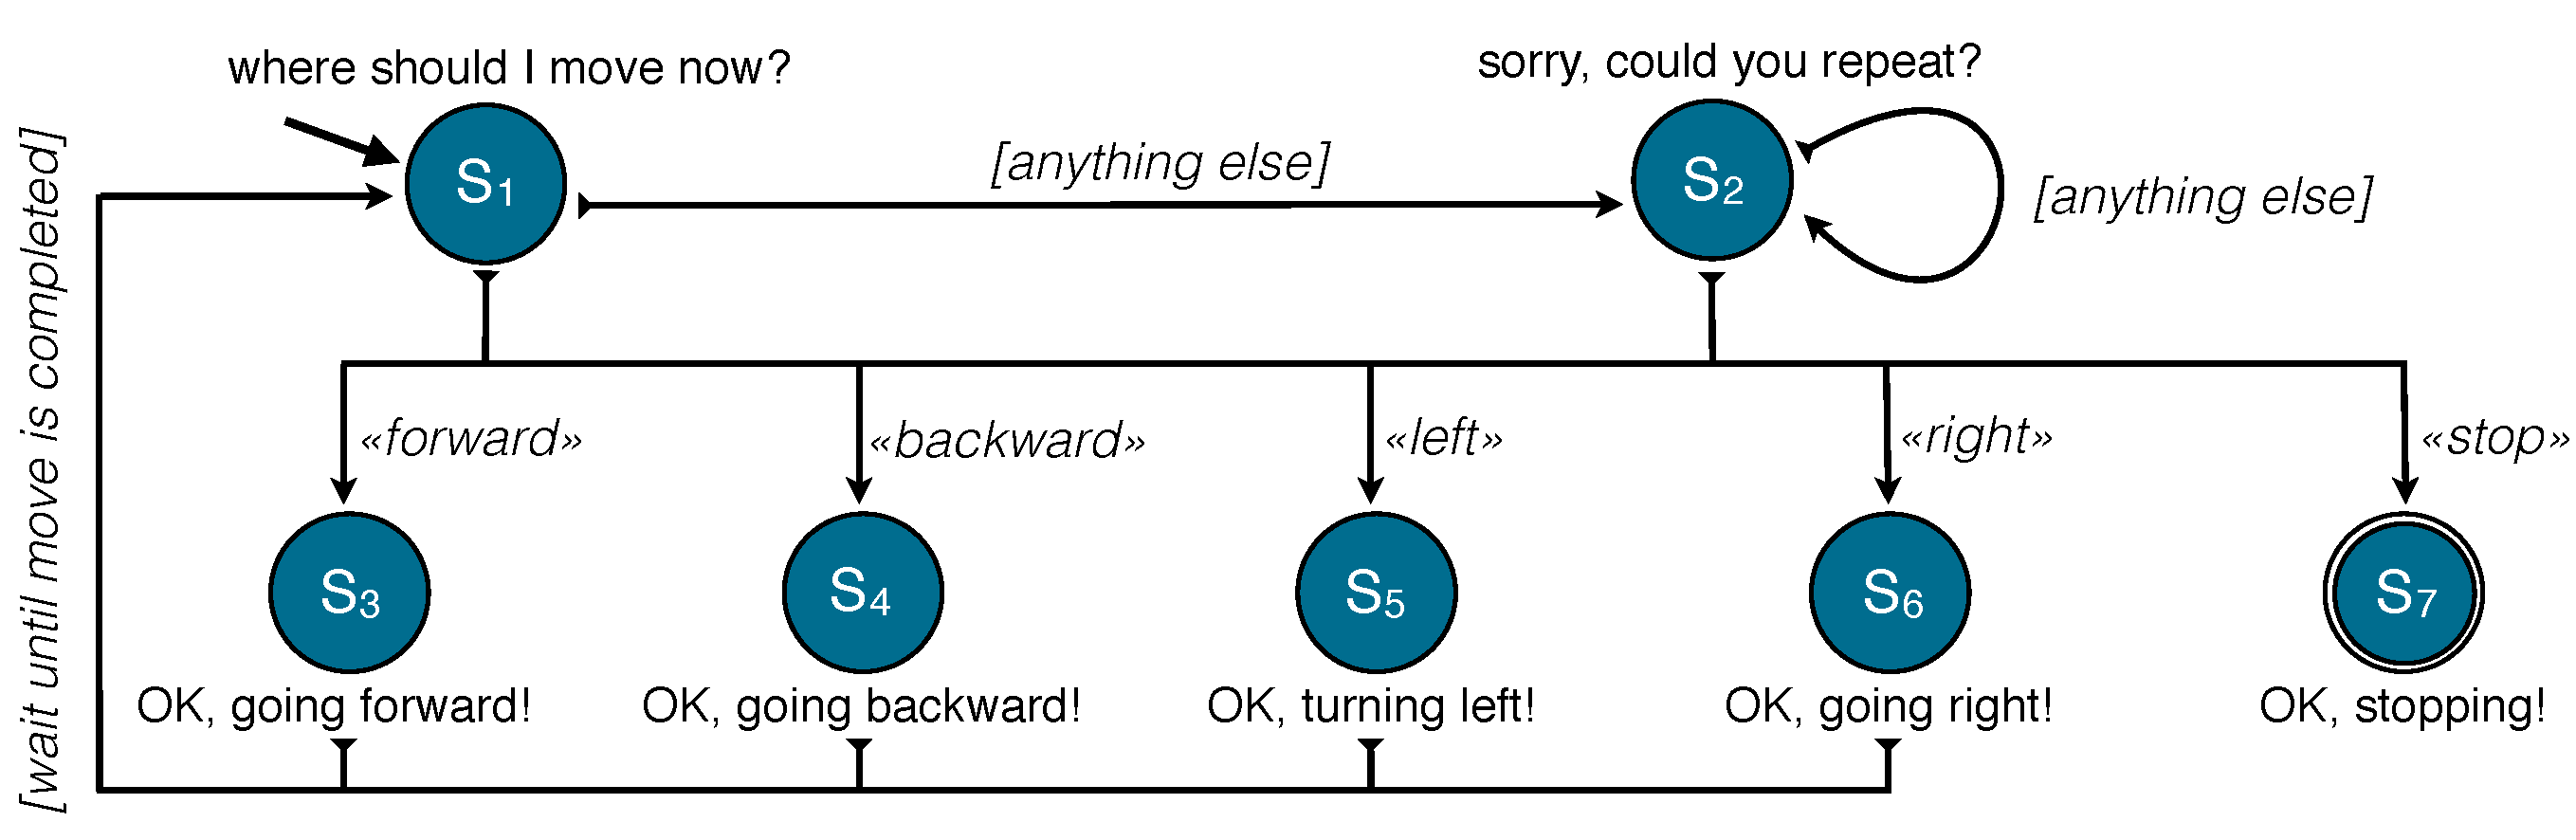
\includegraphics[scale=0.32]{imgs/fsa.pdf}
\caption{Example of finite-state automaton (FSA) for dialogue management, with seven possible states. The starting state for this FSA is $s_1$ and the (unique) ending state is $s_7$. The edges $s_3,... s_7 \rightarrow s_1$ are traversed once the movement is completed, and the two edges $s_1, s_2 \rightarrow s_2$ are traversed for any other user input than the five specified directions.}
\label{fig:fsa}
\end{figure}

A finite-state automaton is formally defined as a tuple $\langle \mathcal{S}, \Sigma, \delta, s_0, \mathcal{F} \rangle$, where $\mathcal{S}$ is the set of possible states, $\Sigma$ the set of inputs that the system can accept (in this case, the user dialogue acts, and possibly external events),  $\delta: \mathcal{S} \times \Sigma \rightarrow \mathcal{S}$ the transition function mapping every (state,input) pair to its successor state, $s_0$ the start state, and $\mathcal{F}$ the set of final states. 

Finite-state automata provide a simple and versatile framework for the development of a dialogue manager. Their expressive power is however rather limited, as the dialogue state of a FSA is represented as a single, atomic symbol, and the possible user moves by a finite enumeration of possible transitions allowed for each state.  Finite-state automata are therefore difficult to scale to more complex domains where the dialogue state might need to track multiple variables and allow for a large number of user dialogue acts.  

\subsubsection*{Logic- and plan-based approaches}

Richer representations of the dialogue state are required to overcome the rigidity of finite-state automata. A popular alternative builds on representations that encode the dialogue state as a frame constituted of a set of slot-value pairs \citep{seneff2000}.  Frame-based systems start with an empty frame that is gradually filled by the user inputs.  After each user move, a set of production rules define what actions to take  -- typically, a request to elicit a value for a particular slot -- based on the current frame.  The process continues until all slots are filled, which marks the completion of the dialogue. 

Due to their greater expressivity, frame-based systems offer a number of advantages in terms of domain modelling and dialogue control.  They remain however difficult to extend to other domains than classical slot-filling applications such as flight booking.  The \textit{information state} approach \citep{Larsson:2000} is an attempt to provide a more solid theoretical foundation for dialogue management in rich conversational domains.  As already mentioned in Section \ref{sec:architectures}, information state approaches rely on a blackboard architecture where various modules are attached to a central workspace called the information state. This information state is therefore continuously monitored by the modules integrated the dialogue system, and represent the full contextual knowledge available to the agent. In addition to the usual variables describing the dialogue history and the application task, the information state can also incorporate ``mentalistic'' entities such as the private and shared beliefs of the conversational agents.  The information state can exhibit a rich internal structure encoded as attribute-value matrices (AVMs) or typed records  \citep{RobinCooper2012}. 

Upon reception of a relevant input, the dialogue manager modifies this information state using a collection of update rules. In addition to state-internal operations that modify particular variables of the information state, the update rules are also employed to derive the actions to execute by the agent.  Given a collection of rules and a generic strategy to apply them, the dialogue manager can both update its state and select the next action to perform by way of logical inference. This action selection can notably be grounded on the set of open questions raised and not yet answered during the interaction \citep{larsson2002,Ginzburg2012}.  

Plan-based approaches such as the ones developed by \cite{Freedman:2000} and \cite{Allen:2001} take one step further. These approaches also rely on complex representations of the dialogue state that notably encompass the belief, desires and intentions (BDI) of each agent \citep{Cohen1979,Allen1980}.  But instead of update rules, classical planning is used to update the state and select the next action.  In such settings, both the user and the system are assumed to act in pursuit of their long term goals.  The interpretation of the user actions is thus cast as a \textit{plan recognition} problem, where the system seeks to derive the belief, desires and intentions that best explain the observed conversational behaviour of the speaker.  Similarly, the selection of system actions is derived from the (task-specific) long term objectives of the system. This search for the best action is an instance of a classical planning task, which can be solved using off-the-shelf planning algorithms. These algorithms require the declaration of a planning domain that specifies the preconditions and effects of every action. Agent-based frameworks such as the Constructive Dialogue Modelling approach developed by \cite{Jokinen:2009} follow similar principles, with a particular emphasis on conceptualising dialogue as a collaborative activity grounded in communicative principles of rational and coordinated interaction between agents. 

\subsubsection*{Benefits and limitations of hand-crafted approaches}

The primary benefits of hand-crafted approaches to dialogue management lie in their ability to capture rich conversational phenomena and endow the system designer with a fine-grained control over the application behaviour.  They have also laid the foundations for substantial advances in the semantic and pragmatic interpretation of dialogue moves \citep{ThomasonManuscript-THOEUA,Ginzburg2012}, the formalisation of social obligations \citep{Traum:1994}, the rhetorical structure of dialogue \citep{0521659515}, or the use of plan-based reasoning to infer the user intentions \citep{Allen1980,Litman87}.  They nevertheless suffer from two important shortcomings: \begin{enumerate}
\item They generally assume complete observability of the dialogue context and provide only a limited account (if any) of uncertainties. This assumption is unfortunately difficult to reconcile with the imperfections and restricted coverage of speech recognition and understanding.
\item They require the dialogue domain to be specified by hand, either through the definition of an finite-state automaton, a collection of update rules or a set of action schemas for planning.  This requirement is hard to satisfy for many domains, since the behaviour of real users is often challenging to anticipate (unsurprisingly, human behaviour can be difficult to predict) and can deviate significantly from the expectations of the system developers. 
\end{enumerate}

Statistical approaches, to which we now turn, have been specifically developed to address these two issues.

\subsection{Statistical approaches}
\label{sec:statistical}

Common to all statistical approaches to dialogue management is the idea of automatically optimising a dialogue policy (that is, a function associating each possible dialogue state to a system action) from interaction data.  Starting from this shared premise, statistical approaches vary along multiple dimensions such as the type of learning algorithm, the representation of the dialogue state and policy, and the nature of the data on which to estimate the models. We outline in this section the core concepts of statistical approaches, which will be exposed in a more formal setting in the next chapter. 

\subsubsection*{Supervised learning}

The first possible approach is to learn dialogue strategies by imitation based on examples of expert behaviour.  This expert behaviour can be recorded through so-called ``Wizard-of-Oz'' experiments.  As already mentioned in the introduction chapter, a Wizard-of-Oz experiment is an interaction in which a human user is asked to interact with a system that is remotely operated by a human agent (without the user being made aware of this control).  A hidden wizard is often preferred to a visible human interlocutor, as people tend to behave differently when they talk to a machine or a human person \citep{JonnsonD88}.  One can collect multiple interactions of this type and record the wizard decisions at each point, along with their context.   The resulting data set can be fed to a supervised learning algorithm in order to construct a dialogue policy that attempts to imitate the conversational behaviour of the wizard.  Learning the dialogue policy is thus seen as a classification problem with states as inputs and actions as outputs. The goal of the learning algorithm is then to construct a classifier  that optimises the classification accuracy for the Wizard-of-Oz data set, considering the wizard actions as ``gold standards''.  This classifier can be estimated with any standard machine learning methods (decision trees, logistic regression, etc.).
 
In a supervised setting, action selection is essentially viewed as a sequence of isolated decision problems.  As argued by \cite{817450}, this formalisation ignores some important characteristics of conversational behaviour. Dialogue is fundamentally a dynamic process where the state and action at time $t$ have a direct influence on the resulting state at time $t+1$.  This temporal connection between states is typically lost with classical supervised learning approaches. Furthermore, the state space grows exponentially with the number of state variables, and can therefore reach very large sizes.  The training data available from a fixed Wizard-of-Oz corpus will therefore only cover a fraction of the state space for the domain.  As a consequence, many states encountered at runtime will have no appropriate training examples on which to ground the action selection.  Generalisation techniques can however be used to mitigate this problem of data sparsity. 

% note about our approach: generalisation enable a better account of the data sparsity problem.  plus, the state dynamics are not lost since we perform belief update.  Finally, the appraoch can be seen as an initial boostrapping that can then be further refined through online reinforcement learning (Bayesian prior), as in Williams etc. also, we learn utilities, not a direct classification. Also: a user simulator is difficulty for situated and open-ended environments.  we learn a POMDP policy by simulation

\subsubsection*{Reinforcement learning}

Reinforcement learning (RL) presents an attractive solution to the problem of dialogue policy optimisation.  A reinforcement learning problem typically revolves around an \textit{agent} interacting with its environment, typically to perform some practical task.  Through its actions, the agent is able to change the state of its environment.  After each action, the agent can observe both the new environment state resulting from its actions, as well as a numerical reward encoding the immediate value (positive or negative) of the executed action in relation to the agent's goal. The goal of the learning agent is to find the best action to execute in any given state via a process of trial and error  -- the best action being characterised as the one that maximise the agent's expected long-term reward.  

Reinforcement learning tasks are generally formalised using \textit{Markov Decision Processes} (MDPs), which are defined as tuples $\langle \mathcal{S}, \mathcal{A}, T, R \rangle$ with a state space $\mathcal{S}$, an action space $\mathcal{A}$, a transition function $T$ that encodes  the probability $P(s'|s,a)$ of reaching state $s'$ after executing action $a$ in state $s$, and a reward function $R$ that specifies the reward value associated with the execution of action $a$ in state $s$. Dialogue can be expressed as a Markov Decision Process where the state space corresponds to the possible dialogue states and the actions to the set of (verbal or extra-verbal) actions available to the dialogue agent.  The transition function $T$ captures the ``dynamics'' of the conversation, and indicates how the dialogue state is expected to change as a result of the system actions. Finally, the reward function $R$ expresses the objectives and costs of the application. A common reward function is to assign a high positive value for the successful completion of the task, a high negative value for a failure, and a small negative value for soliciting the user to repeat or clarify her/his intention.  

Given a particular MDP problem, the goal of the learning agent is to find a policy $\pi: \mathcal{S} \rightarrow \mathcal{A}$ that maps each possible state to the best action to execute at that state.  The best action is defined as the action that maximises the \textit{expected return} for the agent.  Simply put, the return is the long-term (discounted) accumulation of rewards from the current state up to a given horizon. 

Various learning methods have been devised to automatically extract this optimal policy from interaction experience. Due to the large amounts of cycles that are necessary to converge onto an optimal policy, direct interactions with real users are often impossible or highly impractical for many domains. Instead, most recent approaches have relied on the construction of a user simulator able to generate unlimited numbers of interactions on the basis of which the dialogue system can optimise its policy.  
The user simulator can either be designed by experts  or ``bootstrapped'' from existing datasets  or Wizard-of-Oz studies \citep{InTech_RL_2008_OP,FramptonL09}. The reliance on a user simulator for policy optimisation has the major advantage of allowing the learning agent to explore millions of dialogue trajectories on a scale that would be impossible to achieve with real users.  Simulated interactions run however the risk of deviating from real user behaviours.

A limitation faced by MDP approaches is the assumption that the dialogue state is fully observable. As frequently noted in the course of this thesis, this assumption simply does not hold for most dialogue domains, owing to the presence of multiple sources of uncertainty, in particular speech recognition errors.  An elegant solution to this problem is to extend the MDP framework by allowing the state to be a hidden variable that is indirectly inferred from observations.  Such extension gives rise to a  \textit{Partially Observable Markov Decision Process} (POMDP).  POMDPs are formally defined as tuples $\langle \mathcal{S}, \mathcal{A}, T, R, \mathcal{O}, Z \rangle$.  As in a classical MDP, $\mathcal{S}$ represents the state space, $\mathcal{A}$ the action space, $T$ the transition probability $P(s'|s,a)$ between states, and $R$ the reward function $R(s,a)$.  However, the actual state is no longer directly observable.  Instead, the process is associated with an observation space $\mathcal{O}$ that expresses the set of possible observations that can be perceived by the system (for instance, the N-best lists of user dialogue acts generated by the speech recogniser and NLU modules) . The function $Z$ finally defines the probability $P(o|s)$ of observing $o$ in the current state $s$.  

In the POMDP setting, the agent knowledge at a given time is represented by the \textit{belief state} $b$, which is a probability distribution $P(s)$ over possible states.  The belief state is continuously updated as additional information becomes available in the form of e.g. new observations. Based on this belief state, a POMDP policy is defined as a function mapping each possible belief state to its optimal action.  As for MDP-based reinforcement learning, POMDP approaches usually derive the dialogue policy from interactions with a user simulator  \citep{Young:2010,Thomson:2010:BUD:1772996.1773040, daubigney2012}. The optimisation process is however considerably more complex than for MDPs, as the belief state is a continuous and high-dimensional structure. Approximation techniques are therefore necessary in order to extract dialogue policies of reasonable quality in such complex space. The next chapter fleshes out the theoretical foundations of these modelling strategies and their applications to spoken dialogue systems.

\subsubsection*{Benefits and limitations of statistical approaches}

%To conclude this section on statistical approaches to dialogue management, it is useful to recapitulate the major benefits and limitations of statistical approaches compared to the more traditional hand-crafted strategies.  

As stated in the previous sections, one key benefit of statistical approaches is the improved robustness towards errors and unexpected events. This robustness stems primarily from the use of probabilistic reasoning techniques that explicitly account for the uncertainty inherent in spoken dialogue.  The second benefit is the possibility to optimise dialogue policies in a principled, data-driven manner based on a generic specification of the system objectives expressed in the reward function.  This specification allows the system designer to explicitly encode the various goals and costs of the system. This ability to represent trade-offs between multiple, sometimes conflicting objectives is one important advantage of reinforcement learning approaches.  Empirical studies have shown that automatically optimised policies can outperform hand-crafted strategies in both simulated environments and  real user trials, based on objectives and subjective metrics of dialogue success \citep{Supelec270,6407655}. 

Statistical modelling techniques come however with a number of challenges of their own. The most pressing issue is the paucity of appropriate data sets.  Statistical models often require large amounts of training data to estimate their parameters. Unfortunately, real interaction data is scarce, expensive to acquire, and difficult to transfer from one domain to another.  User simulators can partly alleviate this problem, but they must often themselves be bootstrapped from data, and offer no guarantee of producing conversational behaviours that reflect those of real users.  The computational complexity of the learning algorithm can also be problematic. Statistical approaches -- and especially POMDP-based systems -- must often carefully engineer their state and action variables to limit the size of the search space and ensure the learning process remains tractable.  Albeit several dimensionality reduction techniques have been proposed in the literature to address this issue \citep{williams2005,Young:2010,Cuayahuitl:2010,CrookL11}, most work has so far concentrated on slot-filling applications.   Domains such as tutoring systems, cognitive assistants and human-robot interaction must however often deal with state-action spaces that are considerably more elaborate, with multiple tasks to perform, sophisticated user models, and a complex, dynamic environment.  In such settings, the dialogue system might need to track a large number of variables in the course of the interaction, which quickly leads to a combinatorial explosion of the state space.  How to define appropriate statistical models for these open-ended dialogue domains remains an open question, to which the present thesis aims to offer preliminary answers. 

Finally, many practical dialogue applications need to enforce generic constraints on the dialogue flow.  Such constraints may for instance correspond to business rules specific to the particular application.  The incorporation of such constraints in the optimisation process of dialogue policies is however far from trivial. As noted by \cite{Paek:2008}, this lack of direct control on the final policy is one of the main reasons for the slow adoption of RL approaches in industrial systems.  Although some researchers have worked on the integration of expert knowledge into dialogue policy learning \citep{williams2008,Henderson:2008}, much work remains to be done to bring about a unified approach to dialogue management that combines the robustness of data-driven approaches with the control and expressivity of hand-crafted strategies. 

Table \ref{table:approaches} presents a comparison of the most important hand-crafted and statistical methods to dialogue management in terms of state representation, account of state uncertainty (in the sense of having multiple hypotheses about the current state, each one assigned with a specific probability), type of state update and action selection mechanism.  The last row also describes how the approach developed in this thesis stands in comparison to these methods. 
  
\renewcommand{\arraystretch}{2.0}
\setlength{\tabcolsep}{8pt}
\begin{sidewaystable}
\begin{center}
\begin{tabular}{|p{55mm}||p{31mm}|p{16mm}|p{50mm}|p{66mm}|} \hline
\centering \textbf{Approach} &  \centering \textbf{State representation} &  \centering \textbf{State uncertainty} &  \centering \textbf{State update mechanism} & \textbf{Action selection mechanism} \vspace{5pt} \\  \hline \hline
Finite state automata & Atomic state & no & Traversal of matching edge & Action associated with node \vspace{5pt} \\ \hline
Frame-based systems \; \; \; \; \; \; \; \; \; \; \; \; \begin{footnotesize}\citep[e.g.][]{seneff2000}\end{footnotesize}& Slot/value pairs & no & Slot-filling given user inputs & Production rules \vspace{5pt} \\ \hline
Information state update \; \; \; \; \; \; \begin{footnotesize}\citep[e.g.][]{Larsson:2000}\end{footnotesize} & Rich typed feature structure \vspace{5pt} & no & Update rules & Decision rules \vspace{5pt} \\ \hline
Plan-based systems   \; \;  \; \; \; \; \; \; \; \; \begin{footnotesize}\citep[e.g.][]{Freedman:2000,Allen:2001}\end{footnotesize} & BDI model \vspace{5pt} & no & Plan recognition and update of BDI model & Classical planning \vspace{5pt} \\ \hline
Supervised approaches \; \; \; \; \; \; \; \; \begin{footnotesize}\citep[e.g.][]{Hurtado:2005}\end{footnotesize} & Atomic/factored state & no & Extraction of state variables from history and task status & Classifier estimated from Wizard-of-Oz data by supervised learning\vspace{5pt} \\ \hline
MDP-based systems  \; \; \; \; \; \; \; \; \begin{footnotesize}\citep[e.g.][]{Walker:2000,817450}\end{footnotesize} & Atomic/factored state & no & Extraction of state variables from history and task status & Policy optimised via reinforcement learning from real or simulated dialogues \vspace{5pt} \\ \hline
POMDP-based systems \; \; \; \; \; \; \begin{footnotesize}\citep[e.g.][]{Roy:2000,Young:2010}\end{footnotesize}\vspace{5pt} & Atomic/factored state & yes & Update of belief state & Policy optimised via reinforcement learning from real or simulated dialogues \vspace{5pt} \\ \hline
Probabilistic rules & Factored state & yes & Structured belief state update (with probabilistic rules) & Policy optimised via (Bayesian) supervised or reinforcement learning \vspace{5pt} \\ \hline 
\end{tabular}
\end{center}
\caption{Comparison of dialogue management approaches.}
\label{table:approaches}
\end{sidewaystable}


\section{Summary}

We have presented in this chapter the most important concepts and methods in the area of dialogue processing and management.  Starting with a linguistic analysis of the most important dialogue phenomena, we discussed several key aspects of verbal interactions, such as their articulation in sequences of turns and dialogue acts. We also stressed the importance of contextual knowledge in the interpretation and production of dialogue acts, and the role of grounding signals to maintain mutual understanding among the conversational partners. 

Section \ref{sec:sds} described how spoken dialogue systems are internally structured. As we have explained, dialogue systems are often instantiated in complex software architectures that comprise numerous interconnected components for tasks such as speech recognition, understanding, dialogue management, natural language generation and speech synthesis.  Dialogue systems can also be extended to handle (i.e. both perceive and act upon) extra-linguistic modalities and environmental factors. The range of possible applications of dialogue system technology is broad and includes domains as varied as mobile applications for information access and service delivery, in-car navigation systems, smart home environments, cognitive assistants, tutoring systems, and service robots. 

The last section presented an overview of the dialogue management task. A key concept shared by virtually all approaches to dialogue management is the \textit{dialogue state}, a data structure used to encode the system knowledge of the current conversational situation.  This dialogue state can take multiple forms, from the atomic symbols used in finite-state approaches to the rich nested feature structures employed in information state formalisms. Based on this dialogue state, an action selection mechanism is then responsible for the selection of the next action to execute.  In hand-crafted approaches, this mechanism is manually specified by the application developer, either via direct mappings from state to actions, or indirectly through the use of planning techniques.  Statistical approaches, on the other hand, seek to automatically optimise dialogue policies from (real or simulated) interaction data.  A wide range of learning techniques have been developed to perform this optimisation, from supervised learning on a Wizard-of-Oz data set to reinforcement learning based on a user simulator and a generic reward function.   Reinforcement learning techniques can themselves be divided into MDP approaches, where action effects are stochastic but the dialogue state itself is assumed to be known, and POMDP approaches, which incorporate both stochastic action effects and state uncertainty.

We concluded our review of dialogue management approaches by noting that both hand-crafted and statistical methods have significant challenges to address.  This is especially striking for open-ended domains such as human-robot interaction, which exhibit both high levels of noise and uncertainty and a rich dialogue context.   One of the central claims of this thesis is that these domains are best addressed with a hybrid approach to dialogue management that combines probabilistic modelling with expert knowledge about the domain structure.  Chapter \ref{chap:rules} presents how such modelling approach can be formalised.  But before doing so, we first need to lay down the mathematical apparatus required for designing probabilistic models of dialogue, which is the subject of the next chapter.

